\documentclass[a4paper,12pt]{article}
\usepackage[utf8]{inputenc}
\usepackage[cm,empty]{fullpage}
\usepackage[T2A]{fontenc}
\usepackage[english, russian]{babel}
\usepackage{amssymb,amsmath,amsxtra,amsthm}
\usepackage{proof}
\usepackage[pdftex]{graphicx}
\usepackage{wrapfig}
\usepackage{braket}
\usepackage{xcolor}
\usepackage{enumitem}

\usepackage[left=2cm,right=2cm,
    top=1cm,bottom=1cm,bindingoffset=0cm]{geometry}

\renewcommand{\leq}{\leqslant}
\renewcommand{\geq}{\geqslant}


\newcommand{\iiff}{\Longleftrightarrow}
\renewcommand{\iff}{\Leftrightarrow}
\newcommand{\nothing}{\varnothing}

\newtheorem*{rem}{Замечание}

\newcommand{\NN}{\mathbb{N}}
\newcommand{\ZZ}{\mathbb{Z}}
\newcommand{\Q}{\mathbb{Q}}
\newcommand{\A}{\mathbb{A}}
\newcommand{\R}{\mathbb{R}}
\renewcommand{\C}{\mathbb{C}}

\renewcommand{\phi}{\varphi}
\newcommand{\eps}{\varepsilon}

\makeatletter
\newcommand*{\rom}[1]{\expandafter\@slowromancap\romannumeral #1@}
\makeatother

\newcounter{z}


\newcommand{\zs}{\refstepcounter{z}\vskip 10pt\par\noindent
\fbox{\textbf{12.\arabic{z}}} }

\newcommand{\z}{\refstepcounter{z}\vskip 20pt\noindent
\fbox{\textbf{\arabic{z}}} }

\renewcommand{\date}{{\bf 24 мая 2021}} 

\newcommand{\dif}
{
------------------------------------------------------------------------------------------------------------------------------------------------------
}

\newcommand{\HSEhat}{
\vspace*{-0pt}
\noindent
\setcounter{z}{0}


{\bf \phantom{\date}  \large \hfill Теория вероятностей: \hfill \normalsize \date}

\vspace{5 pt}
{\bf \large \hfill  лекция 4\hfill }

\vspace{15 pt}
\centerline{ \large  Домашнее задание.}
\centerline{ \large  Кирилл Сетдеков}



\vspace*{10pt}
\setcounter{z}{0}

}

\begin{document}
\HSEhat


\begin{enumerate}

\subsection*{Задачи:}


\item	При $\lambda > 0$ определим плотность f так: \\
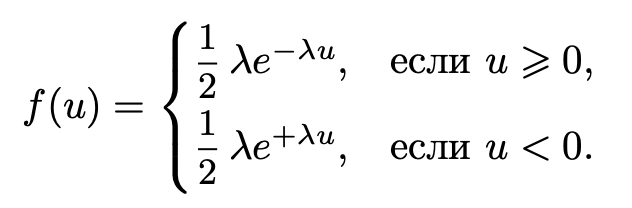
\includegraphics[width=6cm]{img/task1.png}

Такая функция f называется двусторонней экспоненциальной: пусть величина X имеет плотность f. Найдите плотность случайной величины |X|. [Указание. Вычислите сначала функцию распределения.]

\textbf{Решение:}\\
Обозначим $Y\sim |X|$. Посчитаем сначала функцию распределения для $X$:

$$F_{X}(x|x<0)=\int_{-\infty}^{x} \frac{1}{2}\lambda e^{\lambda x} dx = \frac{\lambda}{2} \int_{-\infty}^{x}  e^{\lambda x} dx=\frac{\lambda}{2\lambda}  e^{\lambda x} \Big|_{-\infty}^{x}=\frac{1}{2}  e^{\lambda x}$$
Заметим, что $\int_{-\infty}^{0} f(u) dx =  \int_{-\infty}^{0} \frac{1}{2}\lambda e^{\lambda x} dx= \frac{1}{2} $. Для $x\geq0 \rightarrow \int_{-\infty}^{x} f(u) dx=\int_{-\infty}^{0} f(u) dx+\int^{\infty}_{0} f(u) dx=\frac{1}{2}+\int^{\infty}_{0} f(u)=$
$$=\frac{1}{2}+\int^{\infty}_{0}\frac{1}{2}\lambda e^{-\lambda x} dx=\frac{1}{2}+\frac{\lambda}{2}\int_{0}^{x}  e^{-\lambda x} dx=\frac{1}{2}-[\frac{\lambda}{2\lambda}  e^{-\lambda x} \Big|_{0}^{x}]=\frac{1}{2}+\frac{1}{2}-\frac{1}{2}  e^{-\lambda x}=1-\frac{1}{2}  e^{-\lambda x}$$

У полученной функции $F_X(x) = 1-F_X(-x)$. Распишем, что нам нужно найти: 
$$F_Y(x)=P(|X| <x) = P(x<X<x) = F_X(x)-F_X(-x)=1-F_X(-x)-F_X(-x)=1-2F_X(-x)$$

$$f_Y(x) = F'_Y(x) = -F'_X(-x)=2f_X(-x) =\lambda e^{(-\lambda x)} $$
Действительно, это функция плотности, так как ее интеграл от $-\infty$ до $\infty$ равен 1. $\int_0^{\infty} {\lambda e^{(-\lambda x)} }dx = 1$
 Ниже 0 плотность вероятности 0 так как модуль числа не отрицательный.


\textbf{Ответ:$f_{|X|}(x)=\begin{cases}\lambda e^{(-\lambda x)}, x\geq0 \\
0, x<0\end{cases}$} 


\item	С вероятностью попадания при одном выстреле 0,7 охотник стреляет по дичи до первого попадания, но успевает сделать не более 4 выстрелов. Пусть X - число промахов. Построить таблицу и функцию распределения. 

\textbf{Решение:}\\
Опишем расчет вероятностей:\\
$P(X=0)=1-0.7=0.3$ - мы с 1 выстрела попали\\
$P(X=1)=0.7(1-0.7)=0.21$ - мы с 1 выстрела не попали, но попали со 2\\
$P(X=2)=0.7^2(1-0.7)=0.147$ - мы с 1 и 2 выстрела не попали, но попали с 3\\
$P(X=3)=0.7^3(1-0.7)=0.1029$ - мы с 1 и 2 и 3 выстрела не попали, но попали с 4\\
$P(X=4)=0.7^4=0.2401$ - мы не попали 4 раза\\

$P(X=0)+P(X=1)+P(X=2)+P(X=3)+P(X=4)=1$, запишем найденные вероятности в таблицу, построим функцию распределения, описывая $P(X\leq x)$

\textbf{Ответ:} 

\begin{center}
 \begin{tabular}{|c|c|c|c| c| c |} 
 \hline
 $X$ &0& 1& 2& 3&4\\ [0.5ex] 
 \hline
 $P(X)$& 0,3&	0,21&	0,147&	0,1029&	0,2401 \\ 
 \hline
 $F(X)$ &0,3&	0,51&	0,657&	0,7599	&1  \\ 
 \hline
\end{tabular}
\end{center}

\[
  F(x)=\begin{cases}
               0, x < 0;\\
               0.3, 0\leq x < 1;\\
               0.51, 1\leq x < 2;\\
               0.657, 2\leq x < 3;\\
               0.7599, 3\leq x < 4;\\
               1, x\geq4.
            \end{cases}
\]

\item	Случайная величина X равномерно распределена на отрезке [0, 1]. Докажите, что случайная величина:
 
$$Y = -\frac{1}{\lambda}\ln{(1-X)}$$
имеет экспоненциальное распределение с параметром $\lambda > 0$. Этот факт может использоваться для генерации экспоненциального распределения с помощью равномерного: чтобы сгенерировать экспоненциальную случайную величину можно сгенерировать равномерно распределенную на [0, 1] случайную величину и применить к ней выше приведенное преобразование. 

\textbf{Решение:}\\
Распишем, чем будет функция распределения длс случайной величины $Y$:
$$F_Y(x) = P(-\frac{1}{\lambda}\ln{(1-X)}<x) = P(\ln{(1-X) > -\lambda x})= P(1-X > e^{-\lambda x})=P(-X >-1+e^{-\lambda x})=$$
$$=P(X >1-e^{-\lambda x})$$
Тут $1-e^{-\lambda x} = F_{exp}(x) \in [0,1]$ и при этом $F_Y(0)=0; F_Y(\infty)=1$ и функция $F_Y(x)$ монотонна возрастающая. $F_Y(x)$ удостоверяет требованиям к функции распределения и имеет форму как у экспоненциального распределения.



\item	 Случайные приращения цен акций двух компаний за день X и Y имеют совместное распределение, заданное таблицей:
\begin{center}
 \begin{tabular}{|c| c| c |} 
 \hline
 $X$ \slash $Y$ & $-1$& $+1$ \\ [0.5ex] 
 \hline
 $-1$ & 0,3 & 0,2 \\ 
 \hline
 $+1$ & 0,1	 & 0,4  \\ 
 \hline
\end{tabular}
\end{center}

Найти коэффициент корреляции.

\textbf{Решение:}\\

Для удобства расчета, дополнительно запишем в таблицу вероятности $p(XY), p(X), p(Y)$ и значения $X^2, Y^2$:

\begin{center}
 \begin{tabular}{|c|c|c| c| c |} 
 \hline
 Значение & $p(XY)$& $p(X)$& $p(Y)$&$X^2; Y^2$ \\ [0.5ex] 
 \hline
 $-1$ & 0,3 & 0,5&0,4&1 \\ 
 \hline
 $+1$ & 0,7	 & 0,5&0,6&1  \\ 
 \hline
\end{tabular}
\end{center}
$E(X) = -1 \cdot 0.5 + 1\cdot 0.5=0$\\
$E(Y) = -1 \cdot 0.4 + 1\cdot 0.6=0.2$\\
$E(XY) = -1 \cdot 0.3 + 1\cdot 0.7=0.2$. Вероятности для $XY$ найдены из суммирования вероятностей тех исходов, которые дают произведения $-1$ и $+1$\\
$E(X^2) = 1 \cdot 0.5 + 1\cdot 0.5=1$\\
$E(Y^2) = 1 \cdot 0.4 + 1\cdot 0.6=1$\\

$D(X) = E(X^2)- [E(X)]^2=1-0 = 1$\\
$D(Y) = E(Y^2)- [E(Y)]^2=1-0.04 = 0.96$\\
$Cov(X,Y)=E(XY)-E(X)E(Y)=0.4-0\cdot0.2=0.4$

$$Corr(X,Y) = \frac{Cov(X,Y)}{\sqrt{D(X)D(Y)}}=\frac{0.4}{\sqrt{1\cdot0.96}}\approx 0.40825$$

\textbf{Ответ: Корреляция акций: $Corr(X,Y)\approx 0.40825$} 



\item	Симметричная игральная кость имеет две зеленые, две красные и две белые стороны. Ее подбрасывают один раз. Пусть X = 1, если зеленая сторона сверху и 0 иначе. А Y=1, если красная сторона сверху и 0 иначе. Найдите ковариацию и корреляцию этих случайных величин

\textbf{Решение:}\\
Для удобства расчета, дополнительно запишем в таблицу вероятности $p(X), p(Y)$ и значения $X^2, Y^2, X, Y$:

\begin{center}
 \begin{tabular}{|c|c|c| c| } 
 \hline
 Грань & Вероятность& $X; X^2$& $Y; Y^2$ \\ [0.5ex] 
 \hline
 зеленый & 1/3 & 1&0 \\ 
 \hline
 красный & 1/3	 & 0&1  \\ 
 \hline
 белый& 1/3	 & 0&0  \\ 
 \hline
\end{tabular}
\end{center}

Вероятности выпадения X и Y равны, как и их значения, следовательно:
$E(X)=E(Y)=1\cdot1/3+0\cdot2/3=1/3$\\
$XY=0 \Rightarrow E(XY)=0$\\
$E(X^2)=E(Y^2)=1\cdot1/3+0\cdot2/3=1/3$\\
$D(X)=D(Y)=E(X^2)-[E(X)]^2=\frac{1}{3}-\frac{1}{9}=\frac{2}{9}$\\
$Cov(X,Y)=E(XY)-E(X)E(Y)=0-\frac{1}{3}\frac{1}{3}=-\frac{1}{9}$

$$Corr(X,Y) = \frac{Cov(X,Y)}{\sqrt{D(X)D(Y)}}=\frac{-\frac{1}{9}}{\sqrt{\frac{2}{9}\frac{2}{9}}}=-\frac{\frac{1}{9}}{\frac{2}{9}}=-0.5$$

\textbf{Ответ: $Cov(X,Y)=-\frac{1}{9}\approx-0.11$; $Corr(X,Y)=-0.5$} 

\item	Найдите коэф. Ковариации и корреляции для двух независимых случайных величин $X \sim Exp(3)$ и $X \sim Exp(12)$

\textbf{Решение:}\\
Для удобства, обозначим вторую экспоненциальную случайную величину, как $Y \sim Exp(12)$.
Так как по условию, 2 величины независимы $\Rightarrow E(XY) = E(X)E(Y)$, так как эти 2 величины не зависимы и их вероятности функция плотности совместного распределения их произведения равна произведению функций плотности распределения X и Y. ($g(XY)=f_X(X)\cdot g_Y(Y)$)
$$Cov(X,Y)=E(XY)-E(X)E(Y)=E(X)E(Y)-E(X)E(Y)=0$$
Так как их ковариация равна 0, то разделив ее на $\sqrt{D(X)D(Y)}$, мы также получим также 0 $\Rightarrow Corr(X,Y)=0$

\textbf{Ответ: $Cov(X,Y)=0; Corr(X,Y)=0$} 

\end{enumerate}
\end{document}